% !TeX root = ../praktikum.tex
% !TeX encoding = UTF-8
% !Tex spellcheck = de_DE


Analog zur Auswertung der Gleichstrommessung wurde auch für die aufgenommenen Messdaten der Wechselstrommessung, abgebildet in Graphik \ref{fig:full_range_ac} und \ref{fig:2T_range_ac}, die Dichte der Ladungsträger im 2DEG, sowie deren Beweglichkeit bestimmt.

\subsubsection{Näherung über die Hall-Spannung}
\label{ch:naeherung_hall2}

Wie in der Auswertung der Gleichstrommessung wurde auch hier die Ladungsträgerdichte und deren Beweglichkeit im 2DEG zunächst über die Steigung des klassischen Teils der Hallspannung zwischen \unit[-2]{T} und \unit[2]{T} anhand der Formel $b=\frac{dU_{Hall}}{dB}$  
bestimmt. Dabei ergab sich aufgrund des großen Vorwiderstands ein kleinerer Spannungsabfall relativ zur Spannungsquelle und somit über 
\\
$\frac{dU_{Hall}}{dB}=  \frac{m^2}{s}$  %TODO: ZAHLENWERTE! 
\\
ein geringerer Strom bei der Wechselstrommessung von $I=\unit[]{nA}$. %TODO: ZAHLENWERTE! 

Analog zur Auswertung der Gleichstrommessdaten ergaben sich hier für die gesuchten Größen folgende Werte: \\

$n_s= \frac{1}{cm^2}$  %TODO: ZAHLENWERTE!


$\mu= \frac{cm^2}{Vs}$  %TODO: ZAHLENWERTE! 


\subsubsection{Näherung über die Shubnikov-de Haas-Oszillation}
\label{ch:naeherung_ac}

Ebenfalls analog zur Gleichstrommessung wurden die gesuchten physikalischen Größen alternativ über die Shubnikov-de Haas-Oszillation berechnet. Hierzu wurde wieder die Längsspannung über der Probe 
%$U_{Längs}$
gegen $\frac{1}{B}$ aufgetragen und jedem Minimum der Oszillation ein Füllfaktor $\nu$ zugeordnet. Dies ist in Graphik %TODO: GRAPHIK 
zu sehen. 
Es ergibt sich eine Steigung der Geraden von $b=...$  %TODO: ZAHLENWERTE!
und daraus entsprechend mit Gleichung %TODO: REF
die Ladungsträgerdichte $n_s= \frac{1}{cm^2}$  %TODO: ZAHLENWERTE!
und mit Gleichung %TODO: REF
die Beweglichkeit          
$\mu= \frac{cm^2}{Vs}$ . %TODO: ZAHLENWERTE! 




\begin{figure}[h]
	\centering
	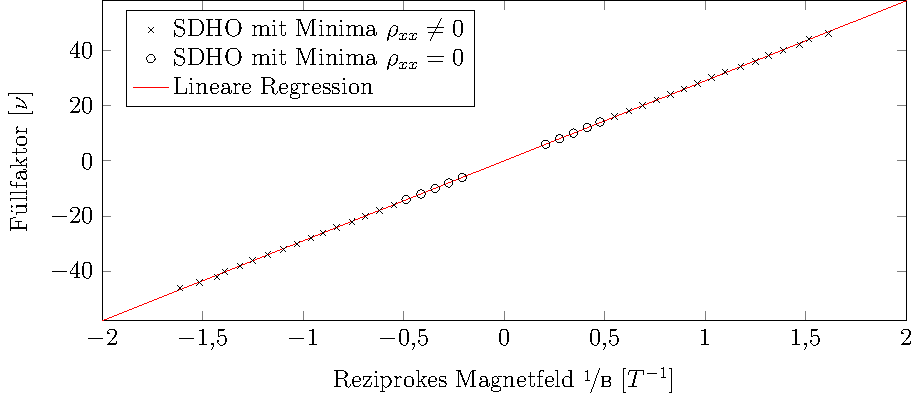
\includegraphics{graphs/ac/auswertung.pdf}
	\caption[Auswertung Füllfaktor Wechselstrommessung]{
		Auswertung Füllfaktor Wechselstrommessung.
	}
	\label{fig:ac_ausw}
\end{figure}

\begin{equation}
\nu= A\cdot x=(28.908\pm 0.035)T \cdot \nicefrac{1}{B}
\end{equation}